
\documentclass[11pt]{article}
\usepackage{hyperref}
\usepackage{makecell}
\usepackage{blindtext}
\usepackage{xcolor}
\usepackage{enumitem}
\usepackage{graphicx,float}
\usepackage{listings}
\hypersetup{
    colorlinks=true,
    linkcolor=blue,
    filecolor=magenta,      
    urlcolor=red,
    pdftitle={Overleaf Example},
    pdfpagemode=FullScreen,
    }
\usepackage{amsmath,amssymb,amsfonts}
\usepackage{graphicx}

\setlength{\topmargin}{-.5in} \setlength{\textheight}{9.25in}
\setlength{\oddsidemargin}{0in} \setlength{\textwidth}{6.8in}

%%%%%%%%%%%%%%%%%%%%%%%%%%%%%%%%%%%%%%%%%%
\usepackage{pythonhighlight}
%%%%%%%%%%%%%%%%%%%%%%%%%%%
\newcounter{mycounter} % create a new counter, called 'mycounter'
% default def'n of '\themycounter' is '\arabic{mycounter}'
%% command to increment 'mycounter' by 1 and to display its value:
\newcommand\showmycounter{\stepcounter{mycounter}\themycounter}
\usepackage{lipsum}
\newcommand\showlips{\stepcounter{mycounter}\lipsum[\value{mycounter}]}
%%%%%%%%%%%%%%%%%%%%%%%%%%%%%%%%%%%%%%
\usepackage{framed}
\usepackage{hyperref}
\usepackage{fancyhdr}

%%%%%%%%%%%%%%%%%%%%%%%%%%%%%%%%%%%%%%%%%%%%%%%%%%%%%%%%%%%%%
\usepackage{listings}
\usepackage{xcolor}

\definecolor{codegreen}{rgb}{0,0.6,0}
\definecolor{codegray}{rgb}{0.5,0.5,0.5}
\definecolor{codepurple}{rgb}{0.58,0,0.82}
\definecolor{backcolour}{rgb}{0.95,0.95,0.92}

\lstdefinestyle{mystyle}{
    backgroundcolor=\color{backcolour},   
    commentstyle=\color{codegreen},
    keywordstyle=\color{magenta},
    numberstyle=\tiny\color{codegray},
    stringstyle=\color{codepurple},
    basicstyle=\ttfamily\footnotesize,
    breakatwhitespace=false,         
    breaklines=true,                 
    captionpos=b,                    
    keepspaces=true,                 
    numbers=left,                    
    numbersep=5pt,                  
    showspaces=false,                
    showstringspaces=false,
    showtabs=false,                  
    tabsize=2
}

\lstset{style=mystyle}
%%%%%%%%%%%%%%%%%%%%%%%%%%%%%%%%%%%%%%%%%%%%%%%%%%%%%%%%%%%%%
\title{\LARGE AI VIET NAM – RESEARCH TEAM}
\author{\Large Towards Learning Universal Hyperparameter Optimizers with Transformers}
\pagestyle{fancy}
\fancyhf{}
\lhead{\bfseries AI VIETNAM}
\rhead{\bfseries  aivietnam.edu.vn}
\begin{document}
\maketitle
%\Largebf Ma 12 Long Test 1\hfill 9 February 2017}
%\medskip\hr
%\noindent{\ule

\begin{enumerate}
    \item
    \textbf{Purpose/outputs:}
    \begin{itemize}
        \item \textbf{OPTFORMER} \cite{https://doi.org/10.48550/arxiv.2205.13320} is a general hyperparameter optimization (HPO) framework based on Transformers \cite{https://doi.org/10.48550/arxiv.1706.03762}. Using a Transformer as a universal interface for modelling experimental data and learn HPO algorithms given a sufficient amount of data, Transformer can potentially learn a more complex prior distribution than standard Bayesian Optimization.
        \item Dealing with large datasets consisting of experimental trials from reality can be challenging, due to large variations in HPO problems and their associated text metadata. Moreover, most meta and transfer-learning HPO methods consider a restrictive setting where all tasks must share the same set of hyperparameters. The authors adopt a supervised learning approach, by learning to predict parameters and hyperparameter response functions from offline tuning data (see \hyperref[fig:optformer]{Figure 1}).\\
        \medskip
        \begin{minipage}{\linewidth}
        \begin{figure}[H]
            \centering
            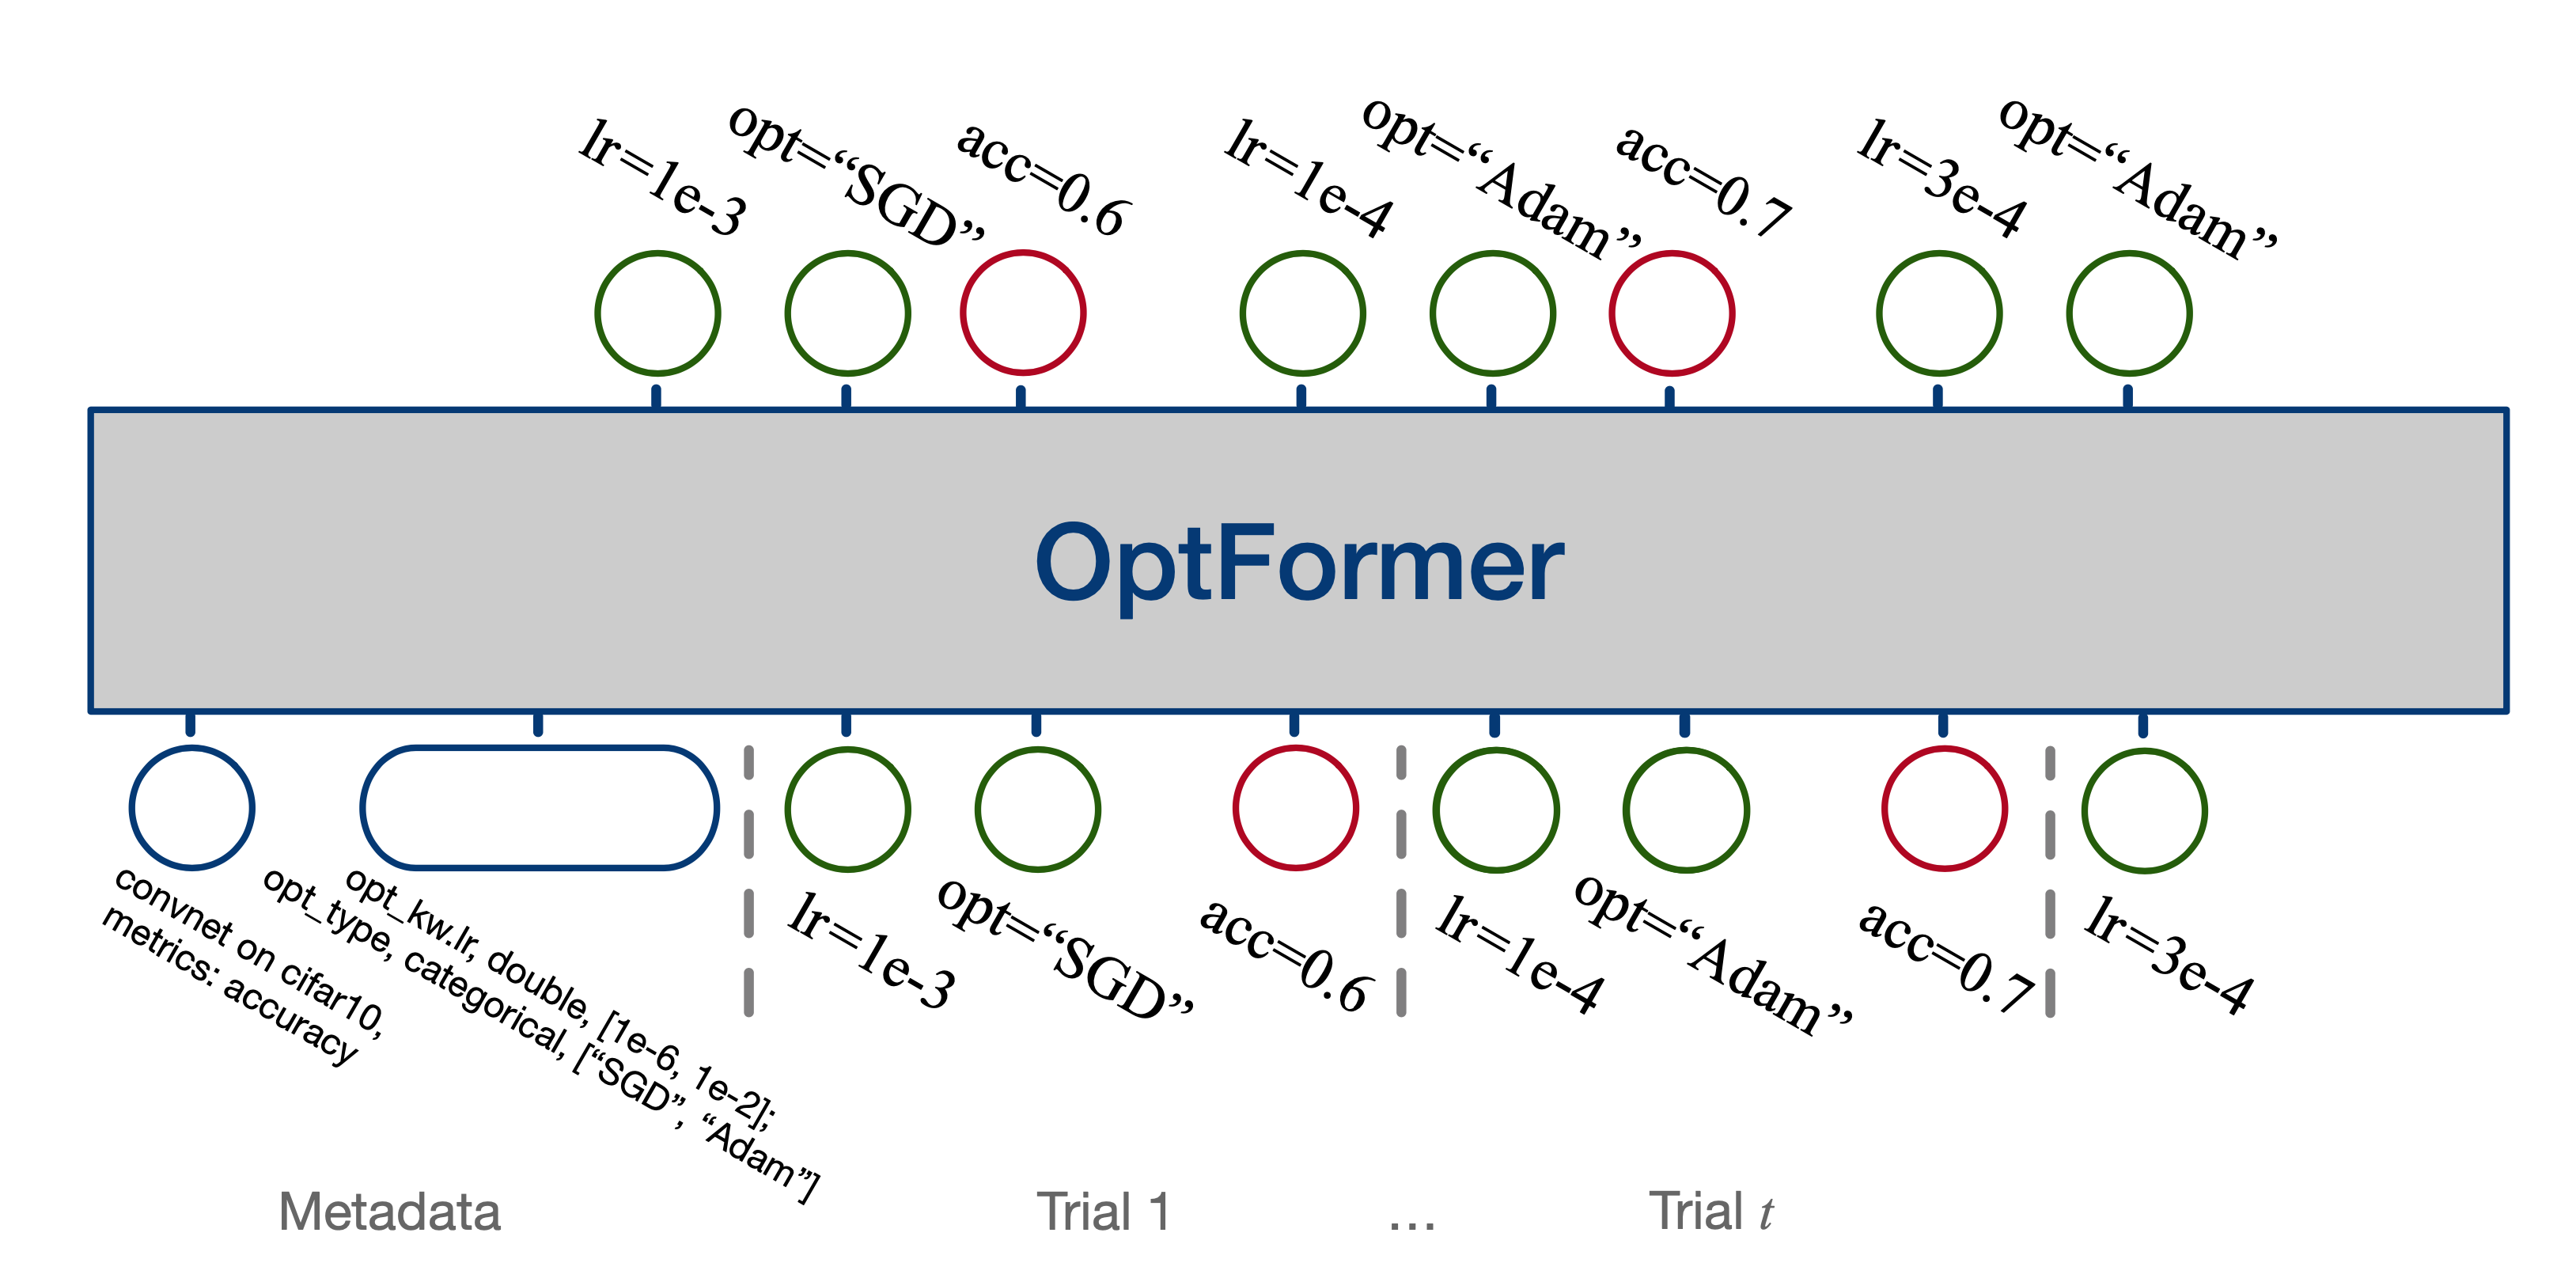
\includegraphics[width=13cm]{optformer.png}
            \caption{Illustration of the OPTFORMER model over a hyperparameter optimization trajectory. It is trained to predict both hyperparameter suggestions (in green) and response function values (in red).}
            \label{fig:optformer}
        \end{figure}
        \end{minipage}
        \end{itemize}
    \item \textbf{Contributions}
    \begin{itemize}
            \item OptFormer makes use of data produced by Google Vizier \cite{46180}, an internal default platform for hyperparameter optimization and overcome drawbacks of previous methods for meta-learning over such data, which includes heavy dependence on numerical constraints and rare usage of textual information.
            \item OptFormer is one of the first Transformer-based frameworks for hyperparameter tuning, learned from large-scale optimization data using flexible text-based representations.
    \end{itemize}
    \item
    \textbf{Methodology:}
    \begin{itemize}
        \item \textbf{Meta-learning for hyperparameter optimization}\\
        HPO aims to find a set of hyperparameters $x$ from search space $\mathcal{X}$ to maximize a model performance metric, $y = f(x)$. The goal of the meta-learning \cite{https://doi.org/10.48550/arxiv.2004.05439} approach for HPO is to learn the shared knowledge among the objective functions $f$ from a dataset of multiple tuning experiments represented as studies and to obtain an optimal HPO algorithm for new hyperparameter tuning tasks from a similar distribution to those in the dataset.\\
        \item \textbf{Representing studies as Tokens}\\
        OPTFORMER takes textual information of study data, including learning rate, optimizer type and accuracy then using concepts from natural language to represents all of the study data as a sequence of tokens. The OptFormer generates new hyperparameters, predicts the task accuracy, and finally receives the true accuracy, which will be used to generate the next round’s hyperparameters. The authors train a 250M parameters T5 \cite{https://doi.org/10.48550/arxiv.2002.08910} on  approximately 200M past training runs from Google’s internal hyperparameter optimization service.\\
        \item \textbf{Inputs tokenization}\\
        All scalar hyperparameters are uniformly quantized to 1000 integer values. Concretely, 
        $$
        \Bar{x} = \text{int}[x_{norm} . Q], \text{where} x_{norm} = (x-x_{min})/(x_{max}-x_{min}) \text{ and } Q = 1000
        $$
        \item \textbf{Intimating policies}\\
        OPTFORMER is trained to predict the next trial in the sequence, which was originally chosen by another HPO algorithm. In other words, the reinforcement learning problem of sequentially choosing the parameters has now become the supervised imitation learning and greedy selection. The OPTFORMER will imitate the algorithm's behavior given text-based prompt in the metadata, as can be seen in \hyperref[fig:result1]{Figure 2}.\\
        \medskip
        \begin{minipage}{\linewidth}
        \begin{figure}[H]
            \centering
            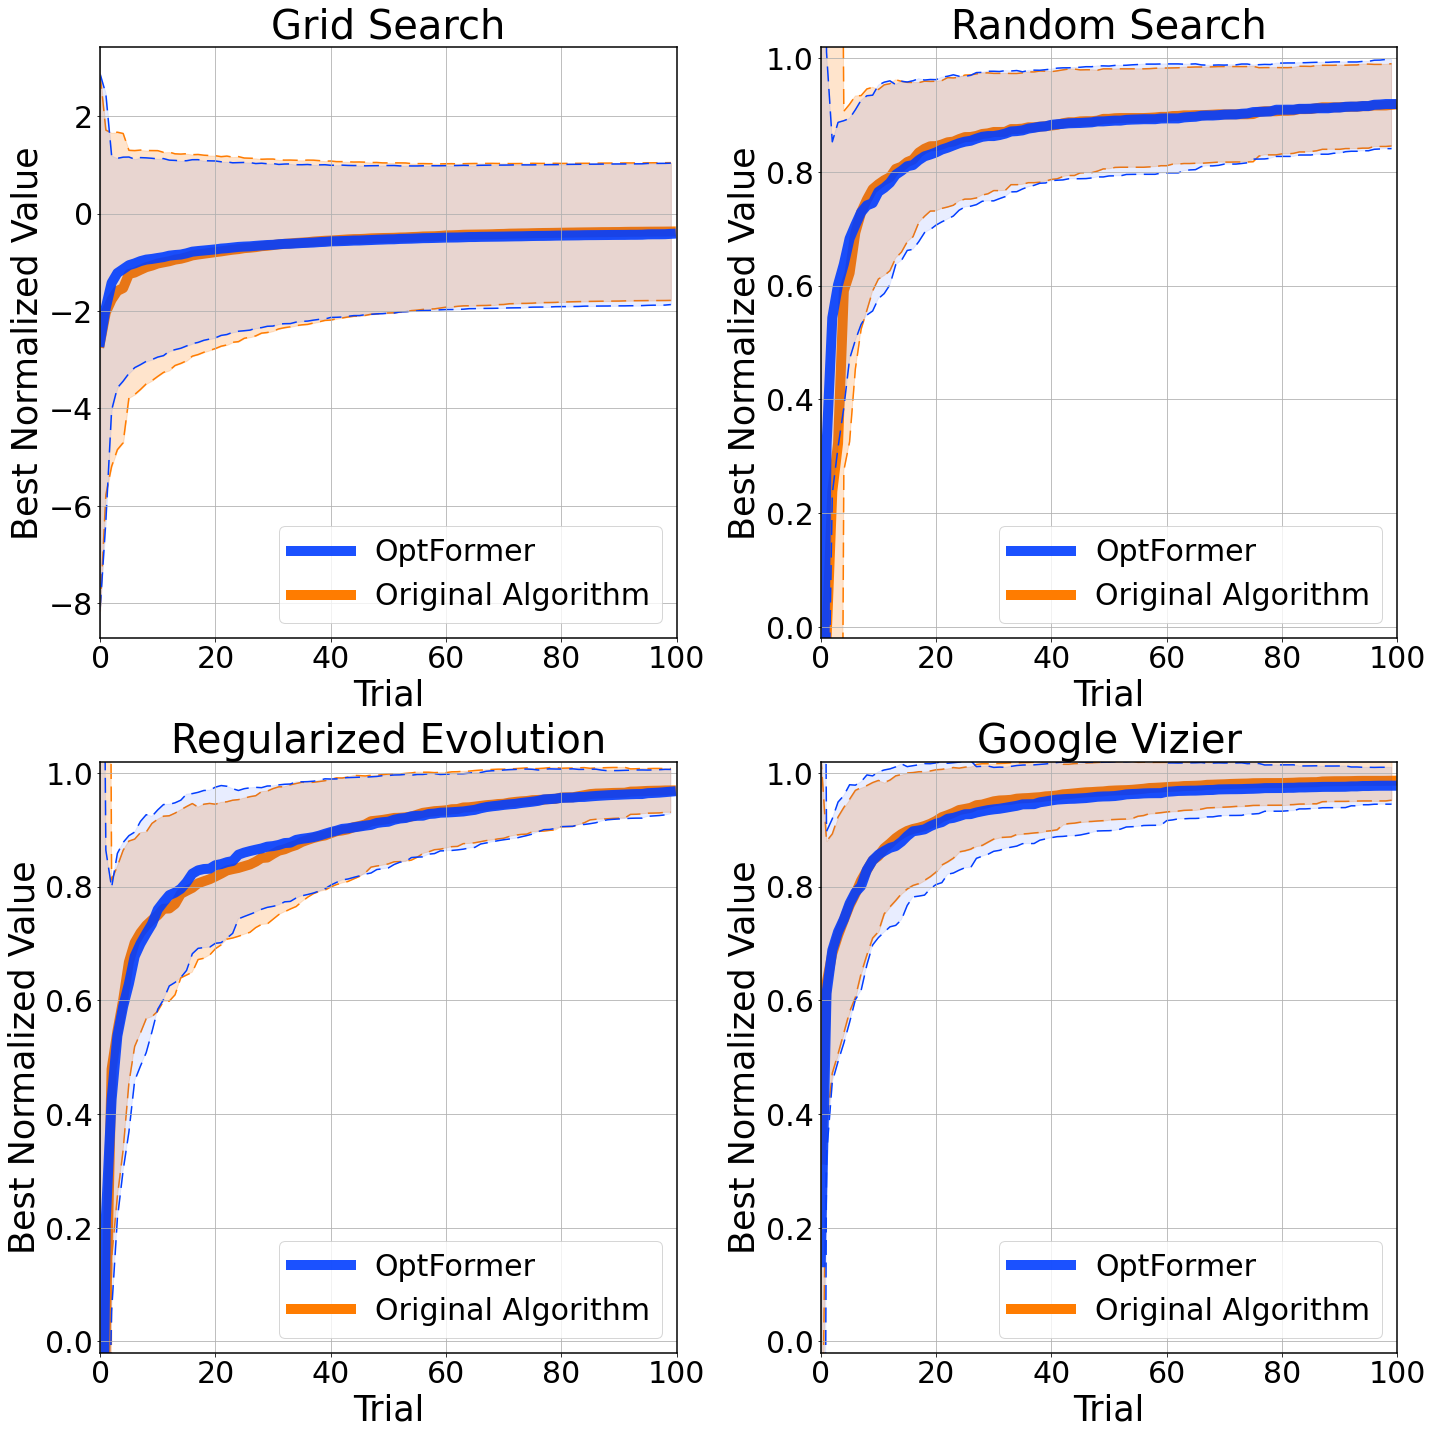
\includegraphics[width=9cm]{image2.png}
            \caption{Over an unseen test function, the OptFormer produces nearly identical optimization curves as the original algorithm. Mean and standard deviation error bars are shown.}
            \label{fig:result1}
        \end{figure}
        \end{minipage}
    \end{itemize}
    \item
    \textbf{Results:}   
    \begin{itemize}
        \item As can be seen in \hyperref[fig:imitating]{Figure 3}, OptFormer imitates most algorithms very accurately in both the mean and variance except for the most complicated algorithm.\\
        \medskip
        \begin{minipage}{\linewidth}
        \begin{figure}[H]
            \centering
            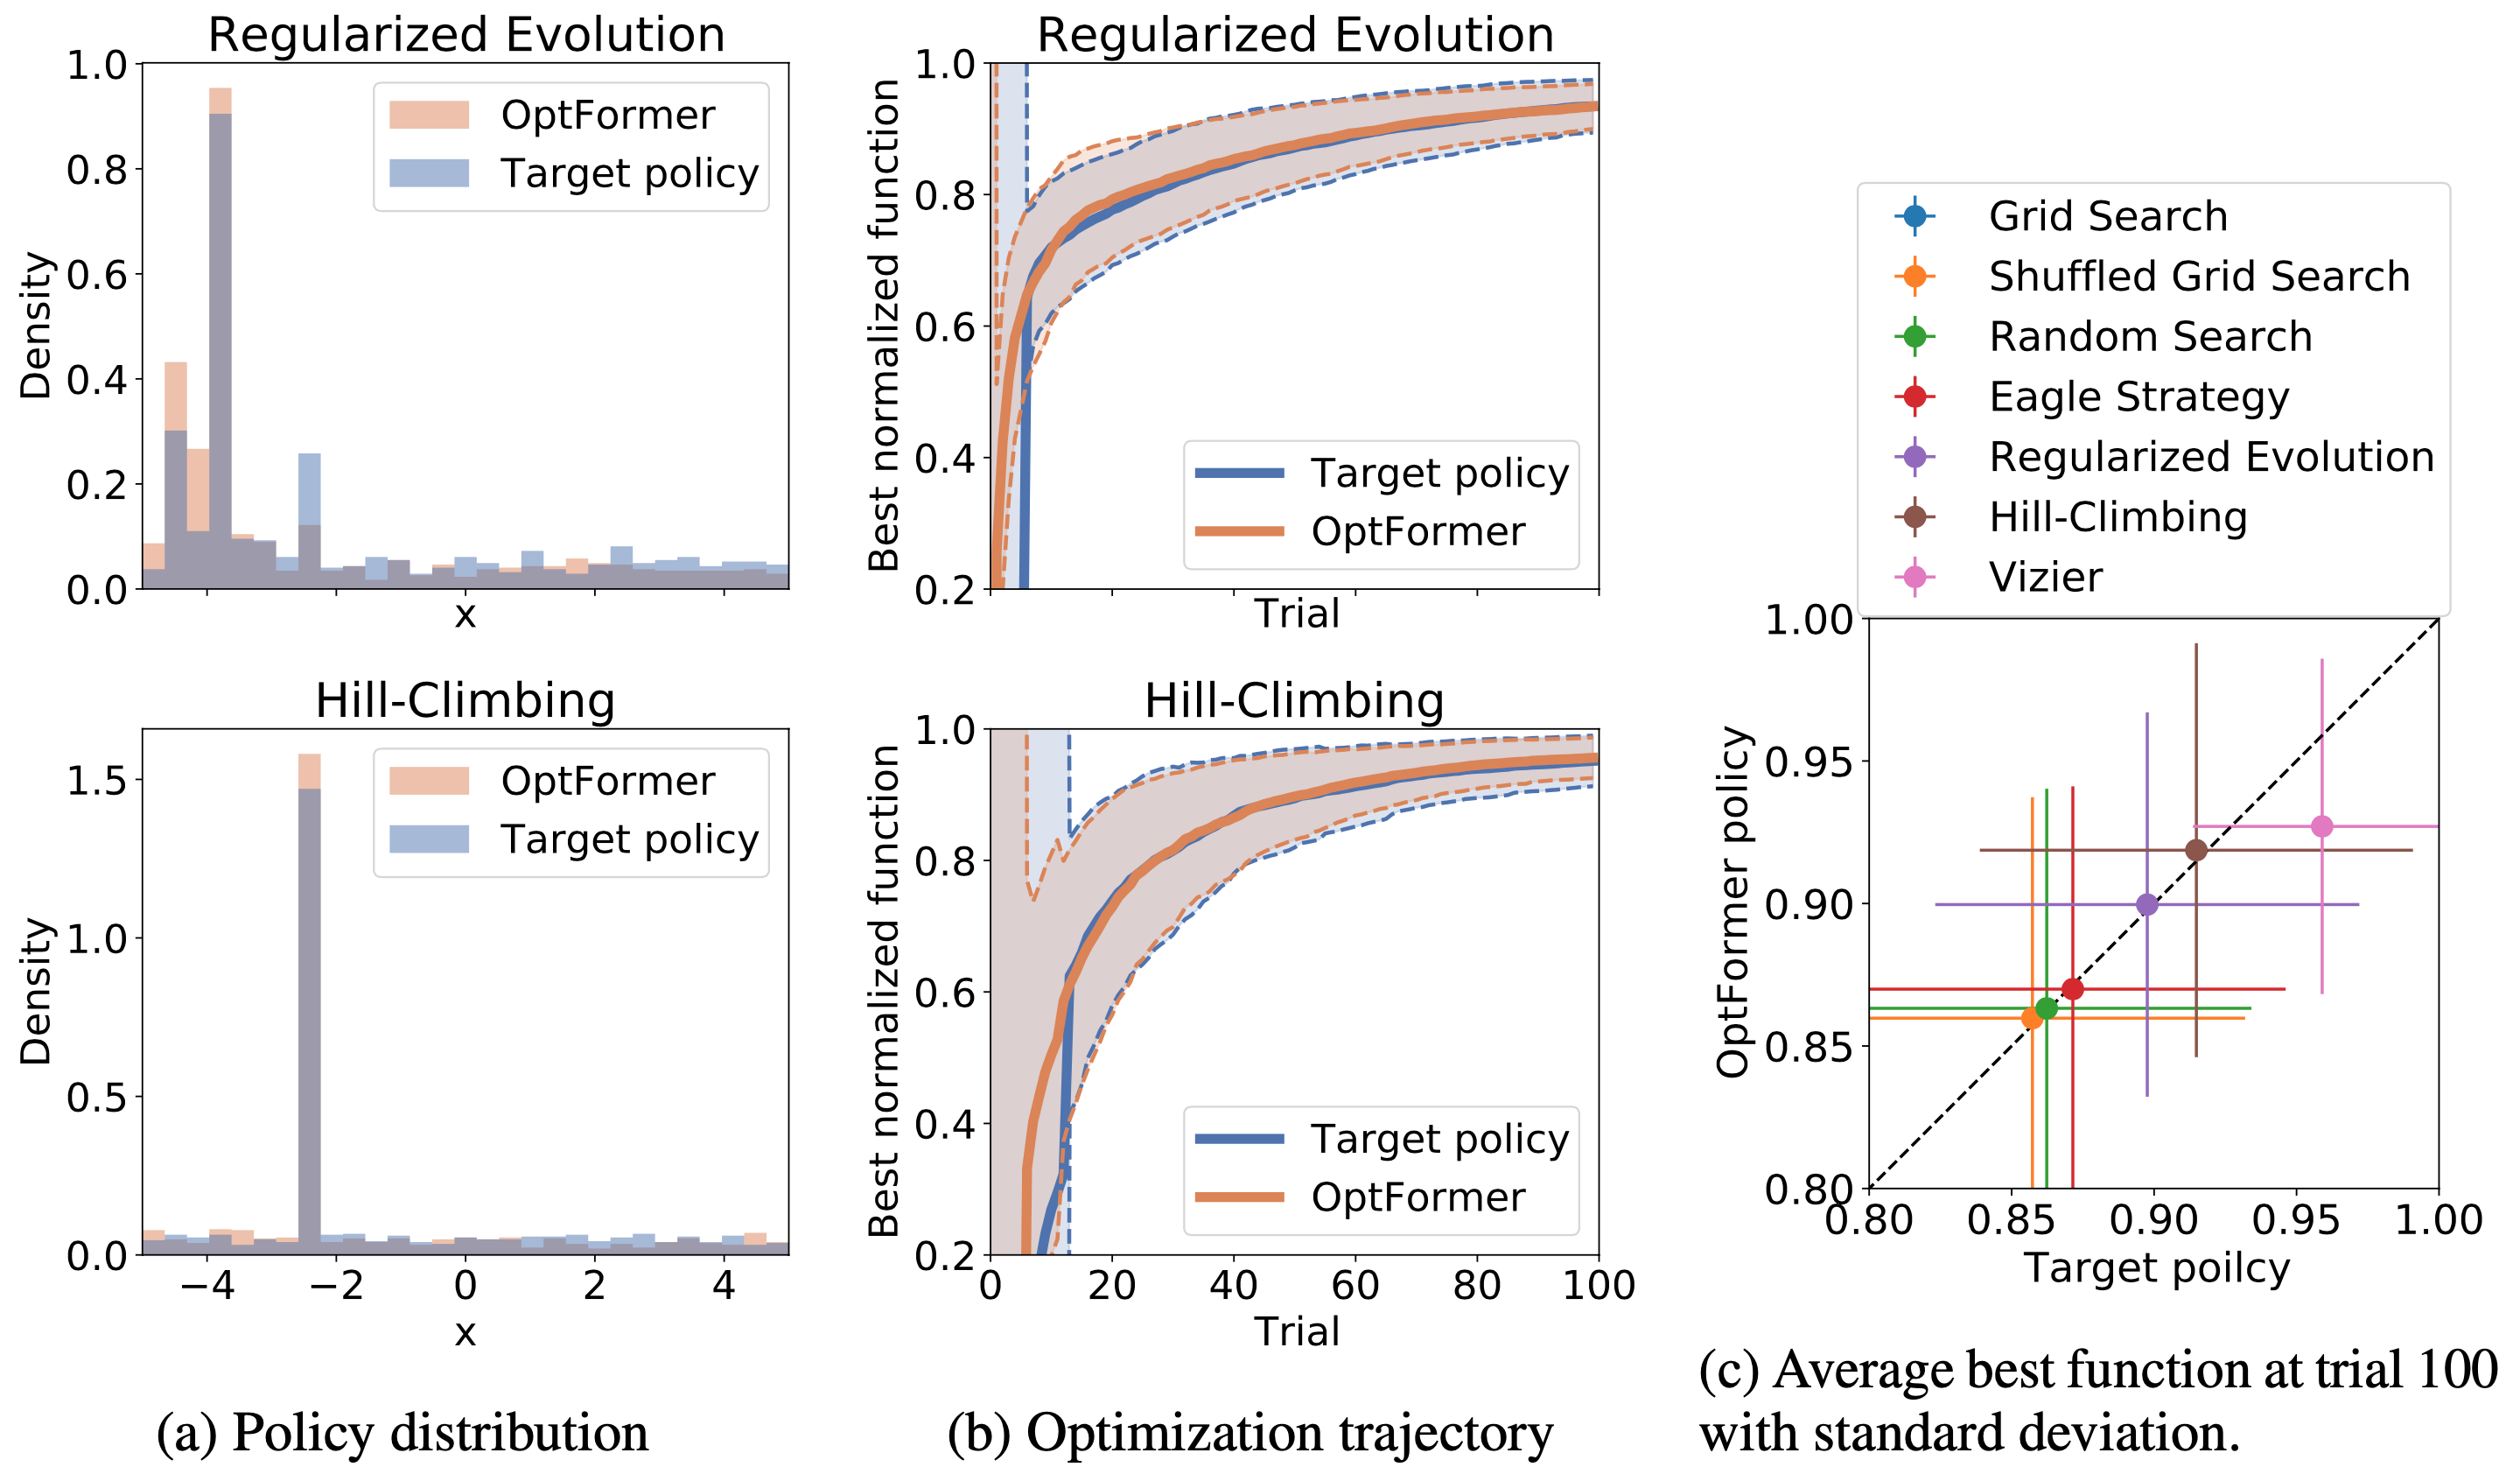
\includegraphics[width=15cm]{r1_1.png}
            \caption{Comparing the performance of different algorithms outputted by the OPTFORMER conditioned on the corresponding algorithm’s name.}
            \label{fig:imitating}
        \end{figure}
        \end{minipage}
        \item The model is capable of predicting objective values very accurately, in many cases surpassing Gaussian Processes, which are commonly used in algorithms such as Bayesian Optimization.\\
        \medskip
        \begin{minipage}{\linewidth}
        \begin{figure}[H]
            \centering
            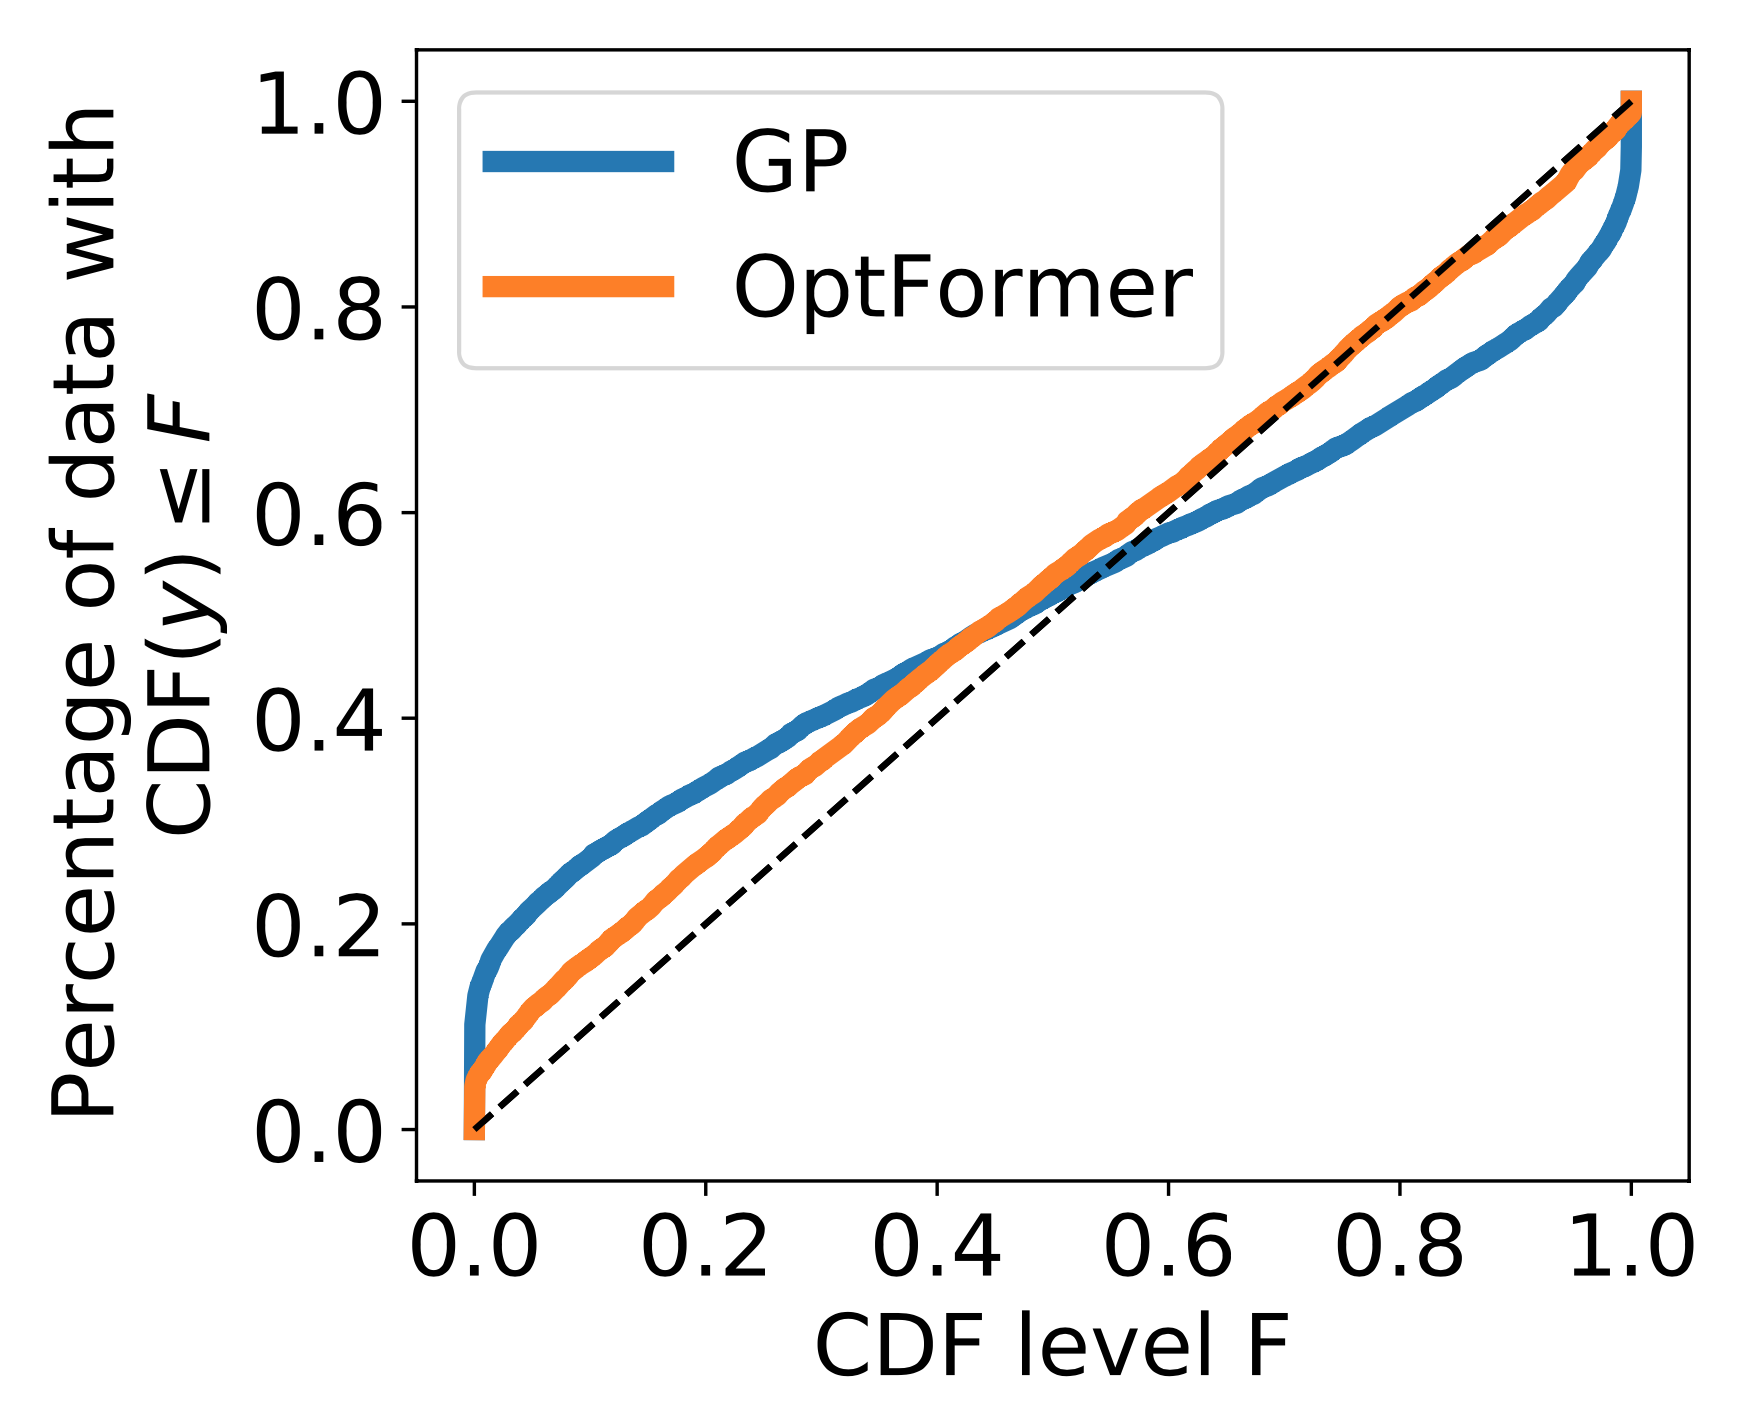
\includegraphics[width=6cm]{r1_2.png}
            \caption{Cumulative histogram of predicted $CDF(y)$ on RealWorldData test set.}
            \label{fig:my_label}
        \end{figure}
        \end{minipage}
        \item The resulting OPTFORMER (EI) outperforms all baselines across the board on both benchmarks when the prior policy is augmented with the Expected Improvement acquisition function.\\
        \medskip
        \begin{minipage}{\linewidth}
        \begin{figure}[H]
            \centering
            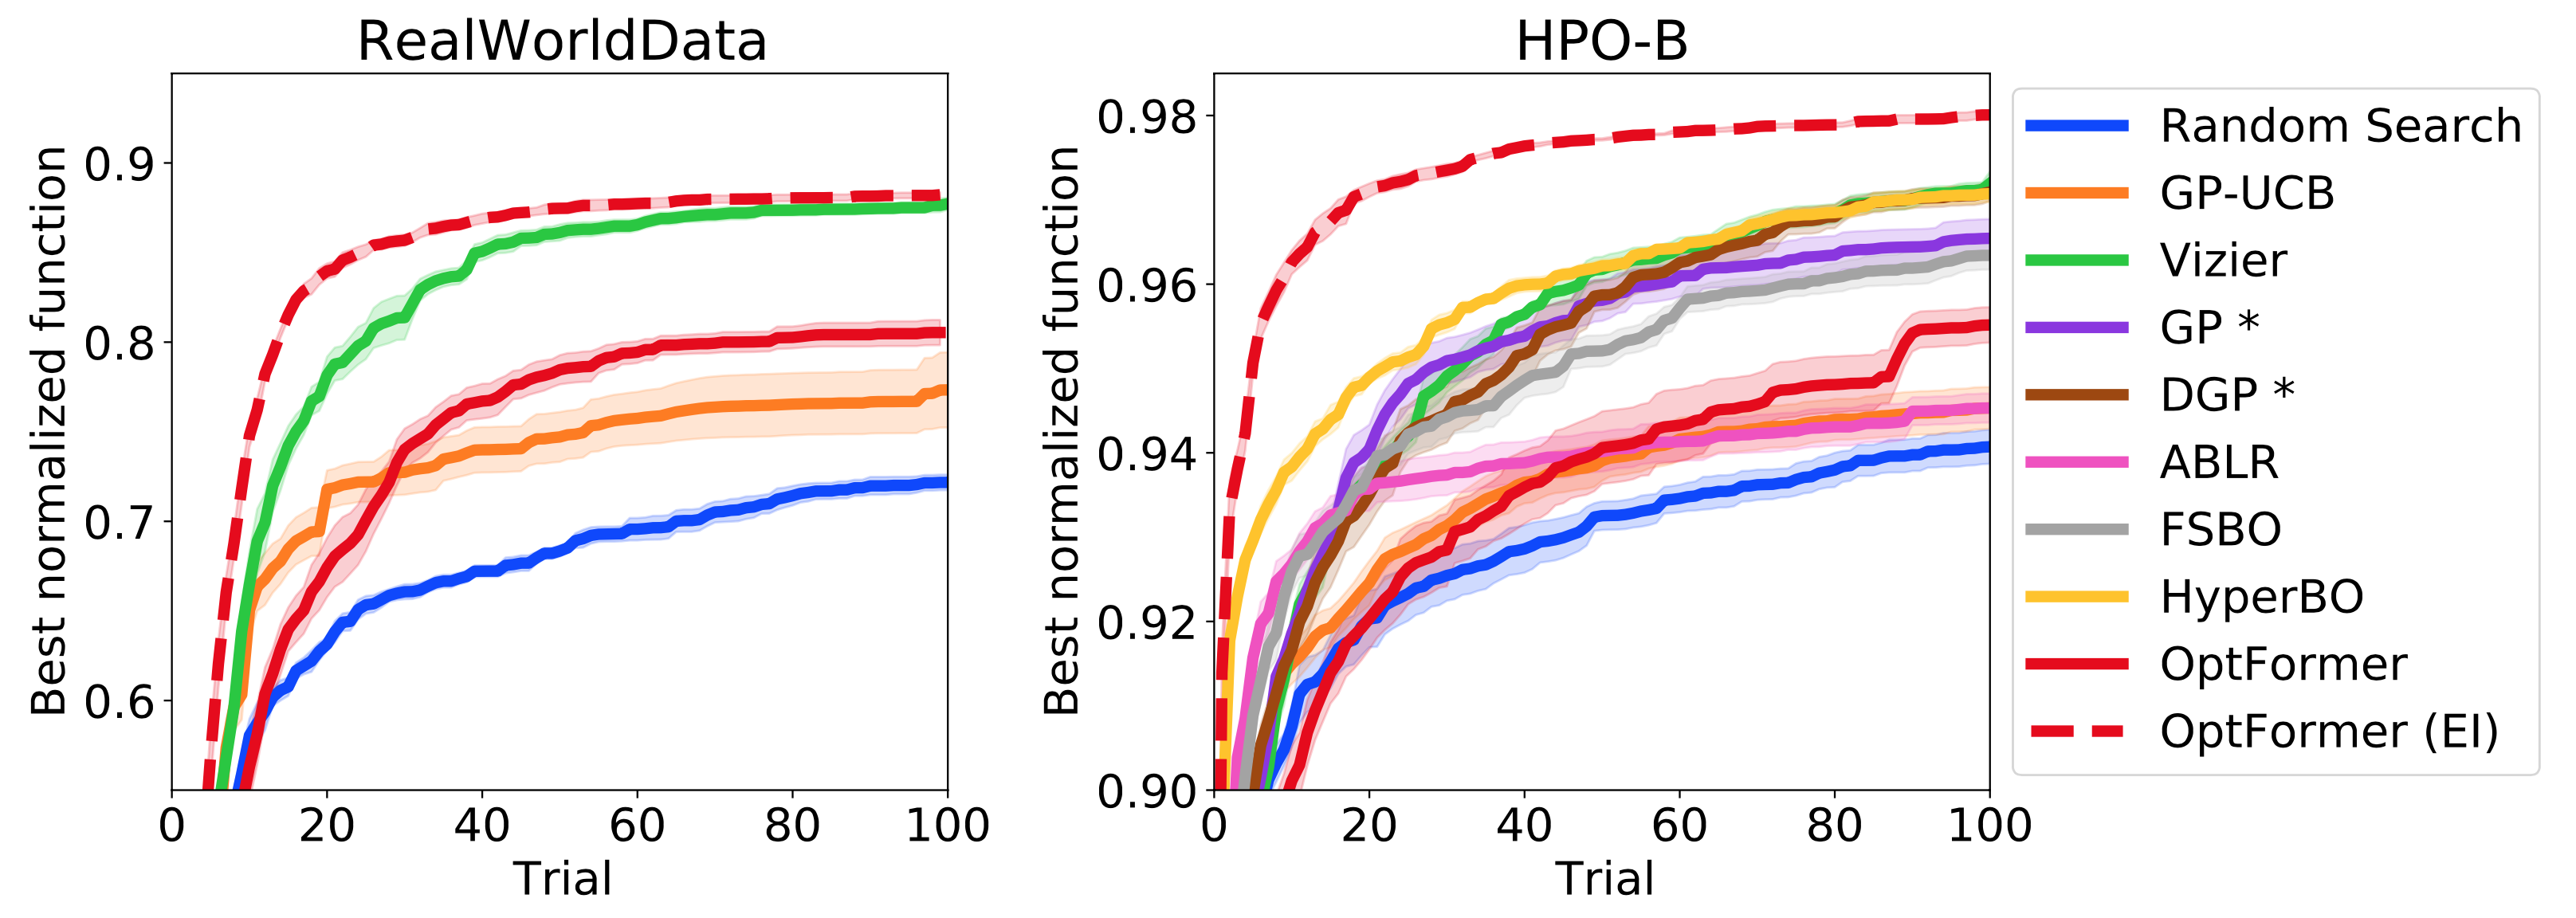
\includegraphics[width=15cm]{r1_3.png}
            \caption{Best normalized function value averaged over 16 RealWorldData test functions (left) and over 86 HPO-B test functions (right) with 1-std confidence interval from 5 runs.}
            \label{fig:my_label}
        \end{figure}
        \end{minipage}
    \end{itemize}
\item \textbf{Limitations}
\begin{itemize}
    \item Parameters that do not always apply or are subject to dynamic constraints depending on other parameter values are not taken into consideration.
    \item Only sequential optimization with a batch size of one are considered.
   \item The authors considered a single objective function while multiple objectives can be easily included by outputting multiple function tokens in a trial. 
    \item The maximum sequence length is limited by the memory size requirement of a Transformer.
\end{itemize}
\item \textbf{Notes}
\begin{itemize}
    \item  Organizations that have trained models will have an advantage when training new ones, suggesting wider adoption of model training services, rather than doing it manually.
    \item In the near future, model training could perhaps consolidate around a few shared services, and rapidly improve in both scale and scope, thanks to ever-larger HPO models.
\end{itemize}
\end{enumerate}
\nocite{*}
\pagebreak
\bibliographystyle{abbrv}
\bibliography{citation}
\end{document} 